\section{Introduction}\label{sec:intro}
%****NOTES START HERE****


%BRAINSTORMING
%\begin{itemize}
%\item Complexity need not be hard to predict (can %point at the simple predictions paper) 
%\item random walk for example is best predicted by %guess what just happend
%\item The kind of complexity present matters, i.e., %that is whether the complexity is structured or not.%






%\item \col brings about the point nicely that some %prediction strategies cannot utilize the processes internal information transfer method. That is a nonlinear internal information transfer system cannot be predicted effectively with a linear strategy. This gives a practitioner leverage on when to give up and when to keep working. 

%\end{itemize}



%\begin{it}
%Paragraph on computer performance, including citations to Todd paper
%and summary of the results that indicate that they're deterministic
%nonlinear dynamical systems.  Given that, we should be able to
%predict.  What benefits would accrue if we could do so: power mgmt,
%end world hunger [this is my primary goal everyday :)], etc.
%\end{it}
%Things to add to introduction
%\begin{enumerate}

%\item \cmark Make an argument that Computer Performance %is a great testing ground as it gives signals that completely cover the spectrum of complexity \col \dots \gcc

%\item When deterministic structure even complex structure exists that structure can be utilized for prediction.
%\item For noisy real-valued time series distinguishing randomness (WN,RW) complexity from structured nonlinear / chaotic /high period / high dimensional etc complexity is (until now) very hard.
%\subitem for this provide predictions of \gcc and \col side by side and discuss "How can we tell if we did a bad job because the method is inadequate vs the signal being too complex. Lead this into is it possible to tell if there exists structure in a time series to know if we should find a better model or not. Maybe even having 4 predictions. top being ARIMA of the above signals and bottom being LMA of the above signals. Show that one improved and one did not. Is it that we used the wrong method to predict or is it that we simply can't predict the signal better than a random walk due to high levels of internal signal complexity.



%\item\cmark Introduce the two main contributions of the paper which are outlined at the begining of the results section

%\end{enumerate}
%\noindent ***NOTES END HERE****
%
%\noindent ****SECTION START****

%<<<<<<< HEAD
%Complicated time-series data are ubiquitous in modern scientific research.  The
%complexity of these data spans a wide %range.  On the low end of this spectrum
%are time series that exhibit perfect %predictive structure, i.e, signals whose
%future values can be successfully %predicted from past values.  Signals like %this
%can be viewed as the product of an %underlying process that generates %information
%and/or transmits it from the past to the %future in a perfectly predictable
%fashion.  Constant or periodic signals, %for example, fall in this class.  On the
%opposite end of this spectrum are signals %that are what we call \emph{fully
%complex}, where the underlying generating %process transmits no information at
%all from the past to the future.  White %noise processes fall in this class.  In
%fully complex signals, knowledge of the %past gives no insight into the future,
%regardless of what model one chooses to %use. Signals in the midrange of this
%spectrum---e.g., deterministic chaos---%pose interesting challenges from a
%modeling perspective.  In these signals, %enough information is being transmitted
%%from the past to the future that an \emph{ideal} model---one that captures the
%generating process---can forecast the future behavior of the observed system
%with high accuracy. Though this notion of complexity differs from that
%considered by e.g. \cite{Shalizi2008}, which would consider a time series
%without any statistical regularities to be non-complex, it has been extensively
%considered by Boffetta et al~\cite{boffetta02}.
%
%As a corollary of the undecidability of the halting
%problem~\cite{halting-problem}, however, no single forecasting schema
%is ideal for all noise-free deterministic
%signals~\cite{weigend93}---let alone all real-world time-series
%data sets.  This leads naturally to an important and challenging
%question: given a complicated real-valued time series, does there
%exist a forecast model that can leverage the information (if any) that
%is being transmitted from past to future by the underlying generating
%process?  A first step in answering this question is to reliably
%quantify where on the complexity spectrum a given time series falls; a
%second step is to determine how complexity and predictability are
%related.  These are the goals of this paper.
%
%In particular, we wish to determine---without knowing anything about
%the generating process---whether a time series is too complex to successfully
%predict.  An important practical corollary to this is a strategy for
%assessing appropriateness of forecast methods.  If the forecast
%produced by a particular method is poor but the time series contains a
%significant amount of predictive structure, one can reasonably conclude that that method is inadequate
%to the task and that one should seek another method.
%=======
Complicated time-series data are ubiquitous in modern scientific
research.  The complexity of these data spans a wide range.  On the
low end of this spectrum are time series that exhibit perfect
predictive structure, i.e, signals whose future values can be
successfully predicted from past values.  Signals like this can be
viewed as the product of an underlying process that generates
information and/or transmits it from the past to the future in a
perfectly predictable fashion.  Constant or periodic signals, for
example, fall in this class.  On the opposite end of this spectrum are
signals that are what one can call \emph{fully complex}, where the
underlying generating process transmits no information at all from the
past to the future.  White noise processes fall in this class.  In
fully complex signals, knowledge of the past gives no insight into the
future, regardless of what model one chooses to use. Signals in the
midrange of this spectrum---e.g., deterministic chaos---pose
interesting challenges from a modeling perspective.  In these signals,
enough information is being transmitted from the past to the future
that an \emph{ideal} model---one that captures the generating
process---can forecast the future behavior of the observed system with
high accuracy. 

% As a corollary of the undecidability of the halting
% problem~\cite{halting-problem}, however, no single forecasting schema
% is ideal for all noise-free deterministic
% signals~\cite{weigend-book}---let alone all real-world time-series
% data sets.  

This leads naturally to an important and challenging question: given a
noisy real-valued empirical time series, does there exist a forecast
model that can leverage the information (if any) that is being
transmitted from past to future by the underlying generating process?
A first step in answering this question is to reliably quantify where
on the complexity spectrum a given time series falls; a second step is
to determine how complexity and predictability are related in these
kinds of data sets.  With these answers in hand, one can develop a
practical strategy for assessing appropriateness of forecast methods
for a given time series.  If the forecast produced by a particular
method is poor, for instance, but the time series contains a
significant amount of predictive structure, one can reasonably
conclude that that method is inadequate to the task and that one
should seek another method.  The goal of this paper is to explore and
formalize that strategy.

% We have two goals in this paper: to determine---without knowing
% anything about the generating process---whether an empirical time
% series is too complex to successfully predict.
%>>>>>>> %1574864f4a0a007a6917eac812688ba02a5de1d5

The information in an observation can be partitioned into two pieces:
redundancy and entropy generation~\cite{crutchfield2003}.
\label{page:redundancy}
Our approach exploits this decomposition in order to assess how much
predictive structure is present in a signal---i.e., where it falls on
the complexity spectrum mentioned above.  We define \emph{complexity}
as a particular approximation of Kolmogorov-Sinai
entropy~\cite{lind95}.  That is, we view a random-walk time series
(which exhibits high entropy) as purely complex, whereas a low-entropy
periodic signal is on the low end of the complexity spectrum.  This
differs from the notion of complexity used by e.g. \cite{Shalizi2008},
which would consider a time series without any statistical
regularities to be non-complex.  We argue that an extension of
\emph{permutation entropy}~\cite{bandt2002per}---a method for
approximating the entropy through ordinal analysis---is an effective
way to assess the complexity of a given time series.  Permutation
entropy is ideal for our purposes because it works with real-valued
data and is known to converge to the true entropy value. Other
existing techniques either require specific knowledge of the
generating process or produce biased values of the
entropy~\cite{bollt2001}.

We focus on real-valued, scalar, time-series data.
%
% that appears complicated: i.e., not periodic, linear, constant, etc.
%
We do not make any knowledge of the generating process or its
properties: whether it is linear, nonlinear, deterministic,
stochastic, stationary, non-stationary, etc.  To explore the
relationship between complexity, predictive structure, and
predictability, we generate forecasts for a variety of time-series
datasets using four different prediction methods, then compare the
accuracy of those predictions to the permutation entropy of the
associated signals.  This results in two primary findings:
\begin{enumerate}
\item The complexity of a noisy real-valued time series is \emph{(i)}
  quantifiable by permutation entropy and \emph{(ii)} correlated with
  the accuracy of an appropriate predictor.
\item The way information is generated and processed internally by a
  system plays a crucial role in the success of different forecasting
  schema---and in the choice of which one is appropriate for a given
  empirical time series.
\end{enumerate}
There has, of course, been a great deal of good work on different ways
to measure the complexity of data, and previous explorations have
confirmed repeatedly that complexity is a challenge to prediction, but
this collection of issues has not been properly explored in the
context of noisy, poorly sampled, real-world data from unknown
systems.  That is the contribution of this paper.

The forecast methods used in this study were chosen to be a
representative sampling of standard prediction strategies, but they do
not, of course, cover that space exhaustively.  Our goal here is an
empirical assessment of the relationship between predictability and
complexity, not formal results about a ``best'' predictor for a given
time series.  From a practitioner's standpoint, it would be useful to
know \emph{ a priori} if a time series contains enough predictive
structure to make it worth spending the time and effort searching for
a good forecast method.  It would also be useful to know if a given
method is inadequate---that is, if an alternative method could do
better and so one should continue searching.

%[Introduce and make it clear why we choose comp. perf. as test bed.]

For the purposes of this study, we require a broad array of
time-series datasets from across the complexity spectrum.  We chose to
study sensor data from a computer-performance experiment.  While this
is not a common laboratory experiment, it is a highly appropriate
choice here.  Computers are extremely complicated systems and their
dynamics is surprisingly rich.
% Modern microprocessor chips contain multiple processing units and
% multi-layer memories, for instance, and they use complicated
% hardware/software strategies to maximize performance by moving data
% and threads of computation across those resources.  As a result, the
The processor and memory loads during the execution of even a very
simple program can exhibit dynamical chaos, for
instance~\cite{mytkowicz09}.  Figure~\ref{fig:col-ipc} shows an
example: a performance trace of a short program that repeatedly
initializes the upper triangle of a matrix in column-major order.
%
 \begin{figure}[htp]
    \centering
    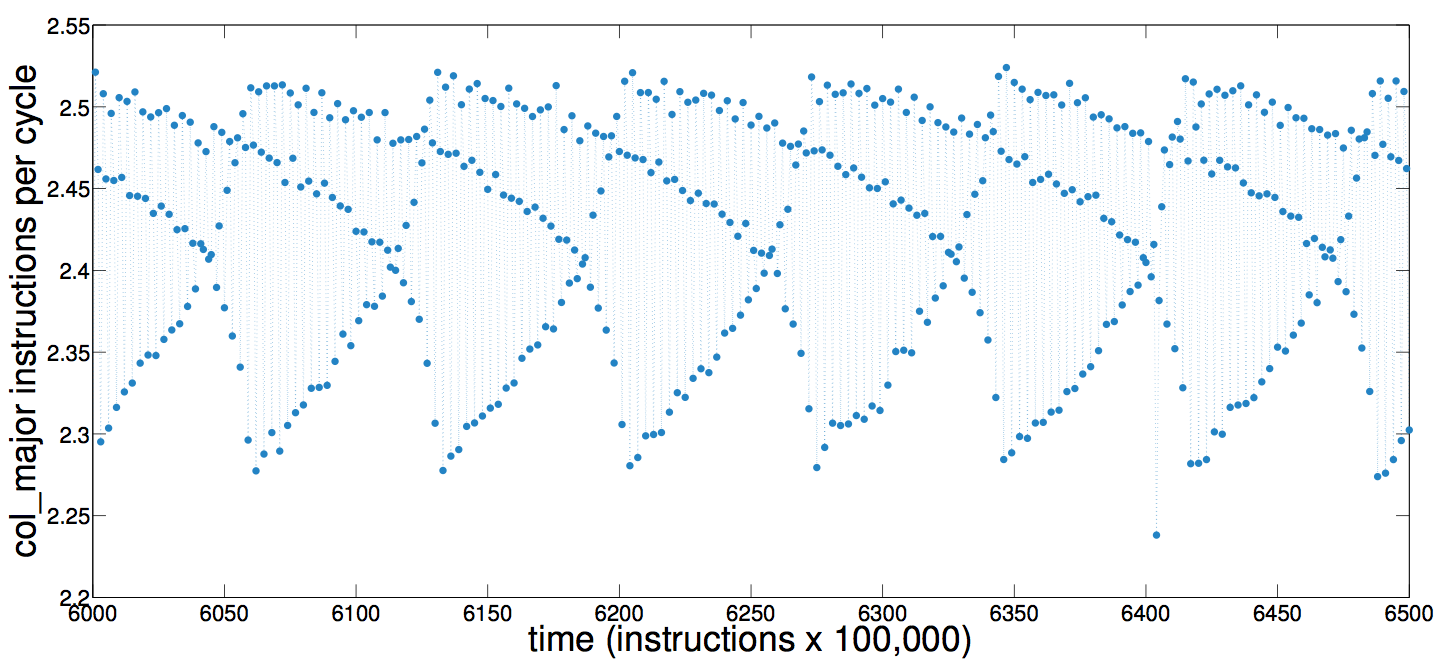
\includegraphics[width=\columnwidth]{figs/colshortts}
    % where an .eps filename suffix will be assumed under latex,
    % and a .pdf suffix will be assumed for pdflatex
    \caption{A computer performance trace: the processor load of \col,
      a simple C program that repeatedly initializes a matrix in
      column-major order, running on an Intel
      i7\textsuperscript{\textregistered}-based machine.}
   \label{fig:col-ipc}
  \end{figure}
%
A small change in the code can cause the dynamics to bifurcate to a
periodic regime.  
% 
% Indeed, many computer performance traces exhibit
% interesting regime changes as a program moves through the different
% phases of its operation.
By running different programs on the same computer, then, we can
produce traces that span the whole range of the complexity spectrum,
from completely predictable to completely unstructured---which makes
this an ideal testbed for this study\footnote{Predicting the
  \emph{state} of a computer, of course, would amount to solving the
  halting problem.  What we are doing here is predicting computer
  \emph{performance}, which does not violate the Rice-Shapiro
  theorem~\cite{hopcroft2007}.}.
% footnote to appease the theoretician in Josh


%The computer systems community has applied a variety of prediction
%strategies to traces like this, most of which employ regression.  An
%appealing alternative builds on the recently established fact that
%computers can be effectively modeled as deterministic nonlinear
%dynamical systems \cite{mytkowicz09}.  This result %implies the
%existence of a deterministic forecast rule for those %dynamics.  In
%particular, one can use \emph{delay-coordinate %embedding} to
%reconstruct the underlying dynamics of computer %performance, then use
%the resulting model to forecast the future values of computer
%performance metrics such as memory or processor loads
%\cite{josh-ida2011}.  In the case of simple microkernels like the one
%that produced the trace in Figure~\ref{fig:ipc}, this deterministic
%modeling and forecast strategy works very well.  In more-complicated
%programs, however, such as numerical software or compilers,
%this forecast strategy---as well as the traditional methods---break
%down some of the time, but work fine others.

%We argue that \emph{permutation entropy}
%\cite{bandt2002per}, a method for measuring the %entropy of a
%real-valued-finite-length time series through ordinal %analysis, is an
%effective way to explore that conjecture.  %{\color{red} Probably remove this and move a%s it is in the experimental methods or point to that section for more details}We study three
%examples---a simple microkernel and two complex %programs: one from the
%SPEC 2006CPU benchmark suite, and one from LAPACK---%running on an Intel i7-based machine.  For
%each program, we calculate the permutation entropy of %the processor
%load (instructions per cycle), then compare that to %the prediction accuracy attainable for
%that trace using a series of deterministic models.

The rest of the paper is organized as follows.
Section~\ref{sec:related} discusses previous results on generating
partitions, local modeling, and error distribution analysis, and
situates this work in that context. Section~\ref{sec:methods} covers
the experimental setup and methods used to collect each time
series. Section~\ref{sec:model} describes the prediction models used
in this study.  Section~\ref{sec:meaComplex} reviews permutation
entropy, the technique that we use to measure complexity.  In
Section~\ref{sec:results}, we estimate the complexity of each
empirical time series and compare that complexity to the accuracy of
predictions produced by the methods of Section~\ref{sec:model},
operating on that time series.  In Section~\ref{sec:conc}, we discuss
these results and their implications, and consider future areas of
research.


